% based on a template made by the university of cologne
% http://www.mi.uni-koeln.de/wp-MIEDV/wp-content/uploads/2016/07/LaTeX-Vorlage.zip - 2023-11-02
\documentclass[12pt,a4paper]{scrartcl}

\addtokomafont{sectioning}{\rmfamily}
\usepackage[ngerman]{babel}% deutsches Sprachpaket wird geladen
\usepackage[T1]{fontenc} % westeuropäische Codierung wird verlangt
\usepackage[utf8]{inputenc}% Umlaute werden erlaubt
\usepackage[usenames]{color} % Erlaubt die Benutzung der namen im Farbpaket und deren Änderung
\usepackage{amsmath} % Erweiterung für den Mathe-Satz
\usepackage{amssymb} % alle Zeichen aus msam und msmb werden dargestellt
\usepackage{graphicx} % Graphiken und Bilder können eingebunden werden
%\usepackage{multirow} % erlaubt in einer Spalte einer Tabelle die Felder in mehreren Zeilen zusammenzufassen
\usepackage{enumerate} % erlaubt Nummerierungen
\usepackage{xurl} % Dient zur Auszeichnung von URLs; setzt die Adresse in Schreibmaschinenschrift.
\usepackage[center]{caption}  % Bildunterschrift wird zentriert
%\usepackage{subfigure} % mehrere Bilder können in einer fugure-Umgebung verwendet werden
%\usepackage{longtable} % Diese Umgebung ist ähnlich definiert wie die tabular-Umgebung, erlaubt jedoch mehrseitige Tabellen.
%\usepackage{paralist} % Modifikation der bereits bestehenden Listenumgebungen
\usepackage{lmodern}% Für die Schrift
\usepackage[hidelinks]{hyperref} % Links und Verweise werden innerhalb von PDF Dokumenten erzeugt
%\usepackage{wrapfig} % Das Paket ermöglicht es von Schrift umflossene Bilder und Tabellen einzufügen.
\usepackage{latexsym} % LaTeX-Symbole werden geladen
\usepackage{tikz} % Erlaubt es mit tikz zu zeichnen
\usepackage{tabularx} % Erlaubt Tabellen
\usepackage{algorithm} % Erlaubt Pseudocode
\usepackage{color} % Farbpaket wird geladen
%\usepackage{stmaryrd} % St Mary Road Symbole werden geladen
\usepackage{physics}
\usepackage{mhchem} % Chemie: \ce & \pu

\numberwithin{equation}{section} % Nummerierungen der Gleichungen, die durch equation erstellt werden, sind gebunden an die section
\newcommand{\HRule}{\rule{\linewidth}{0.7mm}}

\hypersetup{
  pdftitle={B1.5},
  pdfcreator={LaTeX via pandoc}}

\setcounter{secnumdepth}{6}
\setcounter{tocdepth}{6}

\begin{document}
\begin{titlepage}
	\pagestyle{empty}

	\begin{center}

	\textsc{\LARGE Universität zu Köln }\\ [0.4cm]
	\textsc{Mathematisch-Naturwissenschaftliche Fakultät} \\[1.5cm]

	
\includegraphics[width=0.45\textwidth]{../media/uni.jpg}  % Uni-Logo wird geladen

	\textsc{\Large Praktikum~B}\\[2mm]
	\textsc{}\\[10mm]
	\HRule \\[0.4cm]

		{	\Huge \bfseries B1.5}\\[0.4cm]
			{	\huge \bfseries Statistik der Kernzerfälle}\\[0.3cm]
	
	\HRule \\[3cm]

 	\begin{center}
		\textsc{\Large Catherine~Tran } \\[3pt]
		\textsc{\Large Carlo~Kleefisch } \\[3pt]
		\textsc{\Large Oliver~Filla } \\[3pt]
	\end{center}
	\end{center}
\end{titlepage}

\newpage
\tableofcontents
\newpage

\clearpage
\hypertarget{einleitung}{%
\section{Einleitung}\label{einleitung}}

Die Elektronenspinresonanz (ESR) ist eine
Hochfrequenzspektroskopiemethode, welche das Untersuchen von
Eigenschaften paramagnetischer Proben ermöglicht. Sie basiert auf dem
Zeeman--Effekt, der die Aufspaltung von Energieniveaus in einem äußeren
Magnetfeld begründet.

Bei der ESR kann man Übergänge zwischen Zeeman--Niveaus mit gleicher
Hauptquantenzahl beobachten, indem die resonante Absorption von
Mikrowellen beobachtet wird.

Durch das aufgezeichnete Absorptionsspektrum lässt sich weiterhin der
Landé--Faktor bestimmen.

\clearpage
\hypertarget{theoretische-grundlagen}{%
\section{Theoretische Grundlagen}\label{theoretische-grundlagen}}

\hypertarget{magnetismus}{%
\subsection{Magnetismus}\label{magnetismus}}

\hypertarget{dipolmoment}{%
\subsubsection{Dipolmoment}\label{dipolmoment}}

Das magnetische \emph{Dipolmoment} $\vec \mu$ tritt auf, wenn sich
elektrische Ladungen bewegen. Es lässt sich über das auf einen
magnetischen Dipol wirkende Drehmoment $\vec \tau$ in einem Magnetfeld
$\vec B$ definieren.

Für eine ebene Leiterschleife ist es folgendermaßen beschrieben.
\cite{Jackson} Damit ist das Dipolmoment $\vec \mu$ parallel zum
Drehimpuls $\vec{L}$. Die Energie $E$ zur Ausrichtung eines
Dipolmomentes wird durch das Skalarprodukt $\vec \mu \cdot \vec B$
beschrieben.

\begin{eqnarray}
    \vec \tau &=& \vec \mu \times \vec B \\
    E &=& \vec \mu \cdot \vec B
\end{eqnarray}

Das magnetische Moment eines Atoms wird durch Rotation einer
elektrischen Ladung erzeugt. Beispielsweise entsteht im
Bohr--Sommerfeld'schen Atommodell das \emph{Bohr'sche Magneton}
$\mu_B$ durch die Rotation eines Elektrons um den Atomkern. Es wird
durch die reduzierte Planck--Konstante $\hbar$, die Elementarladung
$e$ und die Elektronenmasse $m_e$ beschrieben.

\begin{eqnarray}
    \mu_B &=& \frac{e\hbar}{2m_e}
\end{eqnarray}

\hypertarget{spin}{%
\subsubsection{Spin}\label{spin}}

Der Spin $\vec s$ ist der Drehimpuls, der durch die Rotation eines
Körpers um sich selbst entsteht. Er kann nur einen von zwei Werten
abnehmen.

Beispielsweise beträgt der Eigenwert des Elektronenspins immer
$\pm\frac{\hbar}{2}$, insbesondere gilt für die $z$--Komponente des
Spins $\hat s_3\ket{z\pm}=\pm\frac{\hbar}{2}\ket{z\pm}$. Dadurch ist
die magnetische Quantenzahl $m=\pm\frac{1}{2}$. Da $j$ die Grenzen
der gültigen $m$ definiert, muss die Drehimpulsquantenzahl
$j=s=\frac{1}{2}$ sein. Dies wird als Spin bezeichnet.

Da $s=\frac{1}{2}$ nennt man Elektronen
\emph{Spin-$\frac{1}{2}$--Teilchen} oder Fermionen.

Das Dipolmoment $\vec \mu$ und der Spin $\vec s$ sind über das
\emph{gyromagnetische Verhältnis} $\gamma$ miteinander verknüpft. Dazu
wird der \emph{Landé--Faktor} $g$ benötigt.

\begin{eqnarray}
    \vec \mu &=& \gamma \vec{s} \\
    \gamma &=& \frac{g\mu_B}{\hbar} \\
    g &=& 1 + \frac{j(j+1) + s(s+1) + l(l+1)}{2j(l+1)}
\end{eqnarray}

Hierbei werden die Eigenwerte der Drehimpulsoperatoren
$\hat{\vec j},\hat{\vec s},\hat{\vec l}$ benötigt, die den Spin
$\vec s$, den Bahndrehimpuls $\vec l$ und den Gesamtdrehimpuls
$\vec j = \vec l + \vec s$ beschreiben. Falls es keinen Bahndrehimpuls
$l=0$ gibt, so folgt $g=2$.

\hypertarget{resonanz}{%
\subsection{Resonanz}\label{resonanz}}

Ganz allgemein ist Resonanz das verstärkte Mitschwingen eines
schwingungsfähigen Systems, wenn es einer zeitlich veränderlichen
Einwirkung unterliegt. Dabei kann das System um ein Vielfaches stärker
ausschlagen als beim konstanten Einwirken der Anregung mit ihrer
maximalen Stärke.

Im Falle von ESR werden die magnetischen Dipole von Elektronen resonant
angeregt.

Das magnetische Moment $\mu$ eines Spins im Magnetfeld $\vec{B}$
weist durch Quantenschwebung eine Präzession mit einer
\emph{Lamorfrequenz} $\omega_L$ auf. Dies bedeutet, dass der Spin um
eine Rotationsachse rotiert. Hierbei ist die magnetische Feldkonstante
$\mu_0$ relevant.

\begin{eqnarray}
    \omega_L &=& \frac{2B\mu_0}{\hbar} \\
    \mu_0 &\approx& 4\pi \cdot 1.0 \cdot 10^{-7} \mathrm{\,\frac{Vs}{Am}}
\end{eqnarray}

\hypertarget{zeemanneffekt}{%
\section{Zeemann--Effekt}\label{zeemanneffekt}}

Nach dem Bohr--Sommerfeldschen Atommodell haben Elektronen durch die
Rotation um den Atomkern einen gequantelten Drehimpuls $\vec{L}$. Er
ist durch die Quantenzahl $l=1,2,3,\dots$ quantisiert, es gilt
$|\vec{L}| = l\hbar$. Die Drehimpulskomponente in Richtung der
$z$--Achse $L_z=m\hbar$ ist nun durch eine magnetische Quantenzahl
$m=-l,-l+1,\dots,l$ zu beschreiben.

Durch $L_z$ werden die Energieniveaus der Elektronen verschoben. Diese
Verschiebung führt zu einer Verschiebung der Spektrallinien. Außerdem
ist dadurch auch das magnetische Moment gequantelt.

Der Zeemann--Effekt wird auch Feinaufspaltung genannt.

\hypertarget{chemie}{%
\subsection{Chemie}\label{chemie}}

\hypertarget{radikal}{%
\subsubsection{Radikal}\label{radikal}}

Als Radikale bezeichnet man Atome oder Moleküle mit mindestens einem
ungepaarten Elektron, die meist besonders reaktionsfreudig sind.
Radikale werden mit einem Punkt dargestellt, z.B. Stickstoffmonoxid
$(\ce{NO^\bullet})$, der das freie Elektron symbolisiert.
\cite{Radikale}

Für die ESR ist es wichtig, dass es ungepaarte Elektronen gibt. Daher
werden Radikale benötigt.

\hypertarget{elektrotechnik}{%
\subsection{Elektrotechnik}\label{elektrotechnik}}

\hypertarget{schwingkreise}{%
\subsubsection{Schwingkreise}\label{schwingkreise}}

Ein \emph{$LC$--Schwingkreis} besteht aus einem Kondensator $C$ und
einer Spule $L$, die kurzgeschlossen sind. Die Ladung des Kondensators
wird über die Spule entladen und infolge der Selbstinduktion der Spule
umgekehrt gepolt wieder aufgeladen. Wegen Leitungswiderständen klingt
der Schwingkreis nach wenigen Perioden ab.

\hypertarget{impedanz}{%
\subsubsection{Impedanz}\label{impedanz}}

Die elektrische \emph{Impedanz} ist ein elektrischer Widerstand in der
Wechselstromtechnik. Sie gibt bei einem zweipoligen Netzwerkelement das
Verhältnis von elektrischer Spannung $U$ zur Stromstärke $I$ an.

Der Begriff wird insbesondere dann verwendet, wenn zwischen den beiden
Größen eine Phasenverschiebung besteht, wodurch sich das Verhältnis vom
Widerstand in Gleichstromanwendungen unterscheidet.

Die Impedanz einer Spule $S_L$ wird durch die Induktivität $L$
bestimmt, die Impedanz eines Kondensators $S_C$ durch die Kapazität
$C$.

\begin{eqnarray}
    Z_L &=& i\omega L \\
    Z_C &=& \frac{1}{i\omega C}
\end{eqnarray}

Ein \emph{Ohm'scher Widerstand} ist dagegen ein elektrischer Widerstand,
der unabhängig von elektrischer Spannung $U$, Stromstärke $I$ und
deren Frequenz $\nu$ ist. Das \emph{Ohm'sche Gesetz} kann sowohl für
Ohm'sche Widerstände $R$ als auch für Impedanzen $Z$ angewendet
werden.

\begin{eqnarray}
    U &=& R\cdot I \\
    U &=& Z\cdot I
\end{eqnarray}

\hypertarget{wheatstonebruxfccke}{%
\subsubsection{Wheatstonebrücke}\label{wheatstonebruxfccke}}

Eine \emph{Wheatstonebrücke} wird verwendet, um die ohmschen und
kapazitiven Anteile von Wechselstromwiderständen zu bestimmen.

Dabei werden zwei Wechselstromwiderstände, bestehend aus einem Ohm'schen
Widerstand $R$ und einem Kondensator $C$, in Reihe geschaltet.
Parallel dazu wird ein Widerstand geschaltet, der mit einem Schleifdraht
geregelt werden kann. Dabei ist $R_1$ der Widerstand in der Masche mit
den zu bestimmenden Widerständen $R_x$ und $C_x$, $R_2$ ist der
Widerstand in der Masche mit bekannten Widerständen $R_0$ und $C_0$.

\begin{figure}
	\centering
	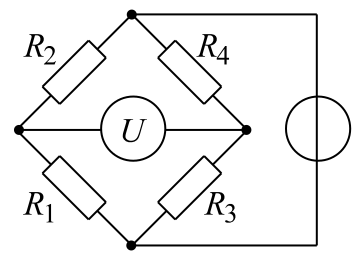
\includegraphics{../media/B1.5/WhBr_Diagonalbild.png}
	\caption{Schaltplan einer Wheatstonebrücke \cite{File:WhBr_Diagonalbild}}
\end{figure}

Durch das Oszilloskopsignal wird der Abgriff des Schleifdrahtes in die
Mitte gebracht. Der Nullabgleich erfolgt dadurch, dass durch eine
geeignete Wahl des Widerstandes $R_0$ und der Kapazität $C_0$ eines
Kondensators das Signal am Oszilloskop auf ein Minimum gebracht wird.
Der Feinabgleich erfolgt mit dem Schleifdraht.

Mithilfe der \emph{Wheatstoneformel} kann ein unbekannter Widerstand
$R_x$ aus drei bekannten Widerständen $R_i$ bestimmt werden.

\begin{eqnarray}
    R_x I_A &=& R_1 I_B \\
    R_0 I_A &=& R_2 I_B \\
    \Rightarrow R_x &=& \frac{R_0\cdot R_1}{R_2}
\end{eqnarray}

\clearpage
\hypertarget{durchfuxfchrung}{%
\section{Durchführung}\label{durchfuxfchrung}}

\clearpage
\hypertarget{auswertung}{%
\section{Auswertung}\label{auswertung}}

\clearpage
\hypertarget{fazit}{%
\section{Fazit}\label{fazit}}

\clearpage
\hypertarget{literatur}{%
\section{Literatur}\label{literatur}}
\renewcommand{\section}[2]{}

\begin{thebibliography}{99}
\bibitem{Uni}
	Universität zu Köln, ``B1.5: Elektronenspinresonanz'', April 2024, Online verfügbar unter 
	\url{https://teaching.astro.uni-koeln.de/sites/default/files/praktikum_b/Anleitung_1.5.pdf}

\bibitem{File:WhBr_Diagonalbild}
	Wikimedia, ``File:WhBr\_Diagonalbild.svg'',
	\url{https://upload.wikimedia.org/wikipedia/commons/e/e3/WhBr_Diagonalbild.svg},
	Abruf am 23.05.2024

\bibitem{Jackson}
	J. D. Jackson, ``Classical Elektrodynamics'', John Wiley \& Sons,
	1975, ISBN 978-0-471-43132-9

\bibitem{Radikale}
	Chemie.de, ``Radikale (Chemie)'',
	\url{https://www.chemie.de/lexikon/Radikale_\%28Chemie\%29.html}, Abruf am 23.05.2024

\end{thebibliography}
\end{document}
